
%% bare_conf.tex
%% V1.4
%% 2012/12/27
%% by Michael Shell
%% See:
%% http://www.michaelshell.org/
%% for current contact information.
%%
%% This is a skeleton file demonstrating the use of IEEEtran.cls
%% (requires IEEEtran.cls version 1.8 or later) with an IEEE conference paper.
%%
%% Support sites:
%% http://www.michaelshell.org/tex/ieeetran/
%% http://www.ctan.org/tex-archive/macros/latex/contrib/IEEEtran/
%% and
%% http://www.ieee.org/

%%*************************************************************************
%% Legal Notice:
%% This code is offered as-is without any warranty either expressed or
%% implied; without even the implied warranty of MERCHANTABILITY or
%% FITNESS FOR A PARTICULAR PURPOSE! 
%% User assumes all risk.
%% In no event shall IEEE or any contributor to this code be liable for
%% any damages or losses, including, but not limited to, incidental,
%% consequential, or any other damages, resulting from the use or misuse
%% of any information contained here.
%%
%% All comments are the opinions of their respective authors and are not
%% necessarily endorsed by the IEEE.
%%
%% This work is distributed under the LaTeX Project Public License (LPPL)
%% ( http://www.latex-project.org/ ) version 1.3, and may be freely used,
%% distributed and modified. A copy of the LPPL, version 1.3, is included
%% in the base LaTeX documentation of all distributions of LaTeX released
%% 2003/12/01 or later.
%% Retain all contribution notices and credits.
%% ** Modified files should be clearly indicated as such, including  **
%% ** renaming them and changing author support contact information. **
%%
%% File list of work: IEEEtran.cls, IEEEtran_HOWTO.pdf, bare_adv.tex,
%%                    bare_conf.tex, bare_jrnl.tex, bare_jrnl_compsoc.tex,
%%                    bare_jrnl_transmag.tex
%%*************************************************************************

% *** Authors should verify (and, if needed, correct) their LaTeX system  ***
% *** with the testflow diagnostic prior to trusting their LaTeX platform ***
% *** with production work. IEEE's font choices can trigger bugs that do  ***
% *** not appear when using other class files.                            ***
% The testflow support page is at:
% http://www.michaelshell.org/tex/testflow/



% Note that the a4paper option is mainly intended so that authors in
% countries using A4 can easily print to A4 and see how their papers will
% look in print - the typesetting of the document will not typically be
% affected with changes in paper size (but the bottom and side margins will).
% Use the testflow package mentioned above to verify correct handling of
% both paper sizes by the user's LaTeX system.
%
% Also note that the "draftcls" or "draftclsnofoot", not "draft", option
% should be used if it is desired that the figures are to be displayed in
% draft mode.
%
\documentclass[conference]{IEEEtran}
% Add the compsoc option for Computer Society conferences.
%
% If IEEEtran.cls has not been installed into the LaTeX system files,
% manually specify the path to it like:
% \documentclass[conference]{../sty/IEEEtran}





% Some very useful LaTeX packages include:
% (uncomment the ones you want to load)


% *** MISC UTILITY PACKAGES ***
%
%\usepackage{ifpdf}
% Heiko Oberdiek's ifpdf.sty is very useful if you need conditional
% compilation based on whether the output is pdf or dvi.
% usage:
% \ifpdf
%   % pdf code
% \else
%   % dvi code
% \fi
% The latest version of ifpdf.sty can be obtained from:
% http://www.ctan.org/tex-archive/macros/latex/contrib/oberdiek/
% Also, note that IEEEtran.cls V1.7 and later provides a builtin
% \ifCLASSINFOpdf conditional that works the same way.
% When switching from latex to pdflatex and vice-versa, the compiler may
% have to be run twice to clear warning/error messages.






% *** CITATION PACKAGES ***
%
\usepackage{cite}
% cite.sty was written by Donald Arseneau
% V1.6 and later of IEEEtran pre-defines the format of the cite.sty package
% \cite{} output to follow that of IEEE. Loading the cite package will
% result in citation numbers being automatically sorted and properly
% "compressed/ranged". e.g., [1], [9], [2], [7], [5], [6] without using
% cite.sty will become [1], [2], [5]--[7], [9] using cite.sty. cite.sty's
% \cite will automatically add leading space, if needed. Use cite.sty's
% noadjust option (cite.sty V3.8 and later) if you want to turn this off
% such as if a citation ever needs to be enclosed in parenthesis.
% cite.sty is already installed on most LaTeX systems. Be sure and use
% version 4.0 (2003-05-27) and later if using hyperref.sty. cite.sty does
% not currently provide for hyperlinked citations.
% The latest version can be obtained at:
% http://www.ctan.org/tex-archive/macros/latex/contrib/cite/
% The documentation is contained in the cite.sty file itself.






% *** GRAPHICS RELATED PACKAGES ***
%
\ifCLASSINFOpdf
  \usepackage[pdftex]{graphicx}
  % declare the path(s) where your graphic files are
  \graphicspath{{../pdf/}{../jpeg/}}
  % and their extensions so you won't have to specify these with
  % every instance of \includegraphics
  \DeclareGraphicsExtensions{.pdf,.jpeg,.png}
\else
  % or other class option (dvipsone, dvipdf, if not using dvips). graphicx
  % will default to the driver specified in the system graphics.cfg if no
  % driver is specified.
  % \usepackage[dvips]{graphicx}
  % declare the path(s) where your graphic files are
  % \graphicspath{{../eps/}}
  % and their extensions so you won't have to specify these with
  % every instance of \includegraphics
  % \DeclareGraphicsExtensions{.eps}
\fi
% graphicx was written by David Carlisle and Sebastian Rahtz. It is
% required if you want graphics, photos, etc. graphicx.sty is already
% installed on most LaTeX systems. The latest version and documentation
% can be obtained at: 
% http://www.ctan.org/tex-archive/macros/latex/required/graphics/
% Another good source of documentation is "Using Imported Graphics in
% LaTeX2e" by Keith Reckdahl which can be found at:
% http://www.ctan.org/tex-archive/info/epslatex/
%
% latex, and pdflatex in dvi mode, support graphics in encapsulated
% postscript (.eps) format. pdflatex in pdf mode supports graphics
% in .pdf, .jpeg, .png and .mps (metapost) formats. Users should ensure
% that all non-photo figures use a vector format (.eps, .pdf, .mps) and
% not a bitmapped formats (.jpeg, .png). IEEE frowns on bitmapped formats
% which can result in "jaggedy"/blurry rendering of lines and letters as
% well as large increases in file sizes.
%
% You can find documentation about the pdfTeX application at:
% http://www.tug.org/applications/pdftex





% *** MATH PACKAGES ***
%
%\usepackage[cmex10]{amsmath}
% A popular package from the American Mathematical Society that provides
% many useful and powerful commands for dealing with mathematics. If using
% it, be sure to load this package with the cmex10 option to ensure that
% only type 1 fonts will utilized at all point sizes. Without this option,
% it is possible that some math symbols, particularly those within
% footnotes, will be rendered in bitmap form which will result in a
% document that can not be IEEE Xplore compliant!
%
% Also, note that the amsmath package sets \interdisplaylinepenalty to 10000
% thus preventing page breaks from occurring within multiline equations. Use:
%\interdisplaylinepenalty=2500
% after loading amsmath to restore such page breaks as IEEEtran.cls normally
% does. amsmath.sty is already installed on most LaTeX systems. The latest
% version and documentation can be obtained at:
% http://www.ctan.org/tex-archive/macros/latex/required/amslatex/math/





% *** SPECIALIZED LIST PACKAGES ***
%
%\usepackage{algorithmic}
% algorithmic.sty was written by Peter Williams and Rogerio Brito.
% This package provides an algorithmic environment fo describing algorithms.
% You can use the algorithmic environment in-text or within a figure
% environment to provide for a floating algorithm. Do NOT use the algorithm
% floating environment provided by algorithm.sty (by the same authors) or
% algorithm2e.sty (by Christophe Fiorio) as IEEE does not use dedicated
% algorithm float types and packages that provide these will not provide
% correct IEEE style captions. The latest version and documentation of
% algorithmic.sty can be obtained at:
% http://www.ctan.org/tex-archive/macros/latex/contrib/algorithms/
% There is also a support site at:
% http://algorithms.berlios.de/index.html
% Also of interest may be the (relatively newer and more customizable)
% algorithmicx.sty package by Szasz Janos:
% http://www.ctan.org/tex-archive/macros/latex/contrib/algorithmicx/




% *** ALIGNMENT PACKAGES ***
%
%\usepackage{array}
% Frank Mittelbach's and David Carlisle's array.sty patches and improves
% the standard LaTeX2e array and tabular environments to provide better
% appearance and additional user controls. As the default LaTeX2e table
% generation code is lacking to the point of almost being broken with
% respect to the quality of the end results, all users are strongly
% advised to use an enhanced (at the very least that provided by array.sty)
% set of table tools. array.sty is already installed on most systems. The
% latest version and documentation can be obtained at:
% http://www.ctan.org/tex-archive/macros/latex/required/tools/


% IEEEtran contains the IEEEeqnarray family of commands that can be used to
% generate multiline equations as well as matrices, tables, etc., of high
% quality.




% *** SUBFIGURE PACKAGES ***
%\ifCLASSOPTIONcompsoc
%  \usepackage[caption=false,font=normalsize,labelfont=sf,textfont=sf]{subfig}
%\else
%  \usepackage[caption=false,font=footnotesize]{subfig}
%\fi
% subfig.sty, written by Steven Douglas Cochran, is the modern replacement
% for subfigure.sty, the latter of which is no longer maintained and is
% incompatible with some LaTeX packages including fixltx2e. However,
% subfig.sty requires and automatically loads Axel Sommerfeldt's caption.sty
% which will override IEEEtran.cls' handling of captions and this will result
% in non-IEEE style figure/table captions. To prevent this problem, be sure
% and invoke subfig.sty's "caption=false" package option (available since
% subfig.sty version 1.3, 2005/06/28) as this is will preserve IEEEtran.cls
% handling of captions.
% Note that the Computer Society format requires a larger sans serif font
% than the serif footnote size font used in traditional IEEE formatting
% and thus the need to invoke different subfig.sty package options depending
% on whether compsoc mode has been enabled.
%
% The latest version and documentation of subfig.sty can be obtained at:
% http://www.ctan.org/tex-archive/macros/latex/contrib/subfig/




% *** FLOAT PACKAGES ***
%
%\usepackage{fixltx2e}
% fixltx2e, the successor to the earlier fix2col.sty, was written by
% Frank Mittelbach and David Carlisle. This package corrects a few problems
% in the LaTeX2e kernel, the most notable of which is that in current
% LaTeX2e releases, the ordering of single and double column floats is not
% guaranteed to be preserved. Thus, an unpatched LaTeX2e can allow a
% single column figure to be placed prior to an earlier double column
% figure. The latest version and documentation can be found at:
% http://www.ctan.org/tex-archive/macros/latex/base/


\usepackage{stfloats}
% stfloats.sty was written by Sigitas Tolusis. This package gives LaTeX2e
% the ability to do double column floats at the bottom of the page as well
% as the top. (e.g., "\begin{figure*}[!b]" is not normally possible in
% LaTeX2e). It also provides a command:
%\fnbelowfloat
% to enable the placement of footnotes below bottom floats (the standard
% LaTeX2e kernel puts them above bottom floats). This is an invasive package
% which rewrites many portions of the LaTeX2e float routines. It may not work
% with other packages that modify the LaTeX2e float routines. The latest
% version and documentation can be obtained at:
% http://www.ctan.org/tex-archive/macros/latex/contrib/sttools/
% Do not use the stfloats baselinefloat ability as IEEE does not allow
% \baselineskip to stretch. Authors submitting work to the IEEE should note
% that IEEE rarely uses double column equations and that authors should try
% to avoid such use. Do not be tempted to use the cuted.sty or midfloat.sty
% packages (also by Sigitas Tolusis) as IEEE does not format its papers in
% such ways.
% Do not attempt to use stfloats with fixltx2e as they are incompatible.
% Instead, use Morten Hogholm'a dblfloatfix which combines the features
% of both fixltx2e and stfloats:
%
% \usepackage{dblfloatfix}
% The latest version can be found at:
% http://www.ctan.org/tex-archive/macros/latex/contrib/dblfloatfix/




% *** PDF, URL AND HYPERLINK PACKAGES ***
%
\usepackage{url}
% url.sty was written by Donald Arseneau. It provides better support for
% handling and breaking URLs. url.sty is already installed on most LaTeX
% systems. The latest version and documentation can be obtained at:
% http://www.ctan.org/tex-archive/macros/latex/contrib/url/
% Basically, \url{my_url_here}.

% \hbadness=99999


% *** Do not adjust lengths that control margins, column widths, etc. ***
% *** Do not use packages that alter fonts (such as pslatex).         ***
% There should be no need to do such things with IEEEtran.cls V1.6 and later.
% (Unless specifically asked to do so by the journal or conference you plan
% to submit to, of course. )


% correct bad hyphenation here
\hyphenation{op-tical net-works semi-conduc-tor}

\usepackage{listings}


\begin{document}
%
% paper title
% can use linebreaks \\ within to get better formatting as desired
% Do not put math or special symbols in the title.
\title{Data management patterns in \\microservices architecture}


% author names and affiliations
% use a multiple column layout for up to three different
% affiliations
\author{\IEEEauthorblockN{Giovanni Jiayi Hu}
\IEEEauthorblockA{Department of Mathematics\\
University of Padua, Italy I-35121\\
Email: giovannijiayi.hu@studenti.unipd.it}}

% conference papers do not typically use \thanks and this command
% is locked out in conference mode. If really needed, such as for
% the acknowledgment of grants, issue a \IEEEoverridecommandlockouts
% after \documentclass

% for over three affiliations, or if they all won't fit within the width
% of the page, use this alternative format:
% 
%\author{\IEEEauthorblockN{Michael Shell\IEEEauthorrefmark{1},
%Homer Simpson\IEEEauthorrefmark{2},
%James Kirk\IEEEauthorrefmark{3}, 
%Montgomery Scott\IEEEauthorrefmark{3} and
%Eldon Tyrell\IEEEauthorrefmark{4}}
%\IEEEauthorblockA{\IEEEauthorrefmark{1}School of Electrical and Computer Engineering\\
%Georgia Institute of Technology,
%Atlanta, Georgia 30332--0250\\ Email: see http://www.michaelshell.org/contact.html}
%\IEEEauthorblockA{\IEEEauthorrefmark{2}Twentieth Century Fox, Springfield, USA\\
%Email: homer@thesimpsons.com}
%\IEEEauthorblockA{\IEEEauthorrefmark{3}Starfleet Academy, San Francisco, California 96678-2391\\
%Telephone: (800) 555--1212, Fax: (888) 555--1212}
%\IEEEauthorblockA{\IEEEauthorrefmark{4}Tyrell Inc., 123 Replicant Street, Los Angeles, California 90210--4321}}




% use for special paper notices
%\IEEEspecialpapernotice{(Invited Paper)}




% make the title area
\maketitle

% As a general rule, do not put math, special symbols or citations
% in the abstract
\begin{abstract}
The microservices architecture is an approach to developing an application as a set of small independent services, which have their own lightweight stack and communicate with other similar services via well-defined interfaces.
In order to achieve loose coupling, a viable strategy is for each service to have its own data store. However, this kind of architecture introduces a new range of obstacles.
We must, indeed, implement transactions that work across multiple distributed services. An operation that spans services must use what’s known as a saga, a message-driven sequence of local transactions, to maintain data consistency. Unfortunately, sagas lack the isolation feature of traditional ACID transactions. As a result, an application must use countermeasures to prevent or reduce the impact of concurrency anomalies caused by the lack of isolation.
On top of that, writing queries in a microservice architecture reveals to be likewise challenging. Implementing queries in an existing monolithic application is relatively straightforward because it has a single database, but in a microservice architecture queries often need to retrieve data that are scattered among the databases owned by multiple services. This paper provides an overview of microservices patterns which emerge when adopting independent data stores, along with some suggested practical implementations.
\end{abstract}

% no keywords




% For peer review papers, you can put extra information on the cover
% page as needed:
% \ifCLASSOPTIONpeerreview
% \begin{center} \bfseries EDICS Category: 3-BBND \end{center}
% \fi
%
% For peerreview papers, this IEEEtran command inserts a page break and
% creates the second title. It will be ignored for other modes.
\IEEEpeerreviewmaketitle



\section{Introduction}
A microservice is as a small self-contained application that has a single responsibility, a lightweight stack, and can be deployed, scaled and tested independently \cite{exploring-microservices}. Services run in their own remote processes and communicate between each other using a lightweight mechanism such as message-queuing, which is discussed later. 

The central aspect of the microservice definition is the independence, the ability for a service to change without affecting any other. As such, services are indipendently deployable and scalable in addition to offering a better fault isolation than the monolithic architecture. For example a memory leak in one service will only affect that service, while the other ones will continue to handle the requests normally.

To achieve this praised independence, the database architecture must respect the following requirements:

\begin{itemize}
  \item Services must be loosely coupled so that they can be developed, deployed and scaled independently;
  \item Some business transactions must enforce invariants that span across multiple services. For instance, before placing an order, you must verify that a new order will not exceed the customer’s credit limit;
  \item Some business transactions need to query data that are owned by multiple services. For example, displaying the orders require querying the Orders service to gather the cost and the Restaurant service to know if an order has been accepted;
  \item Different services might have different data storage requirements. For an Orders service a relational database could be the best choice, but other services might need a SQL database with extensions for non-relational features, such as geospatial datatypes, or even a NoSQL database. A service which provides the nearest restaurants certainly requires geospatial queries.
  \item Databases must support replication and sharding in order to scale. Replication improves the application availability and performance whereas sharding allows the application to handle increasing data volumes;
  \item Databases contain no business logic, such as stored procedures. In doing so, databases for different services can more easily combined and separated with minimal code changes \cite{ebay-architecture}.
\end{itemize}

A standard solution to these requirements is to keep each microservice’s persistent data private to that service and accessible only via its API. The transactions of a service involve only its database. 
Using a database per service allows the services to be loosely coupled and guarantees higher resilience. Changes to one service’s database do not impact any other services. Besides, each service can use the type of database that is best suited for its needs. For example, a service that handles text searches could use ElasticSearch \cite{database-per-service}.

However, using a database per service introduces severe drawbacks which must be carefully evaluated: implementing business transactions that span across multiple services is complex and implementing queries which join data from several databases is challenging.

\section{Queries}

Three problems are commonly encountered when implementing queries in a microservice architecture:

\begin{enumerate}
  \item To perform a single task, a client may have to make multiple calls to various  services, which result in high latency and poor user experience. This chattiness between a client and different services can adversely impact the performance and scale of the application;
  \item Retrieving data scattered across multiple services can result in expensive, inefficient in-memory joins without a proper solution;
  \item The service can store the information in a database that doesn’t efficiently support the required query, for instance traditional relational databases are not efficient for geospatial queries.
\end{enumerate}

\subsection{API composition pattern}

The most straightforward approach is the API composition pattern \cite{microservices-patterns-api-composition}, which implements a query operation by invoking the services that own the data and combining the results. As example, a query operation to show the details of an order might invoke three services - \texttt{Order Service, Delivery Service and Payment Service} - and return aggregate the results.

\begin{figure}[!htbp]
\centering
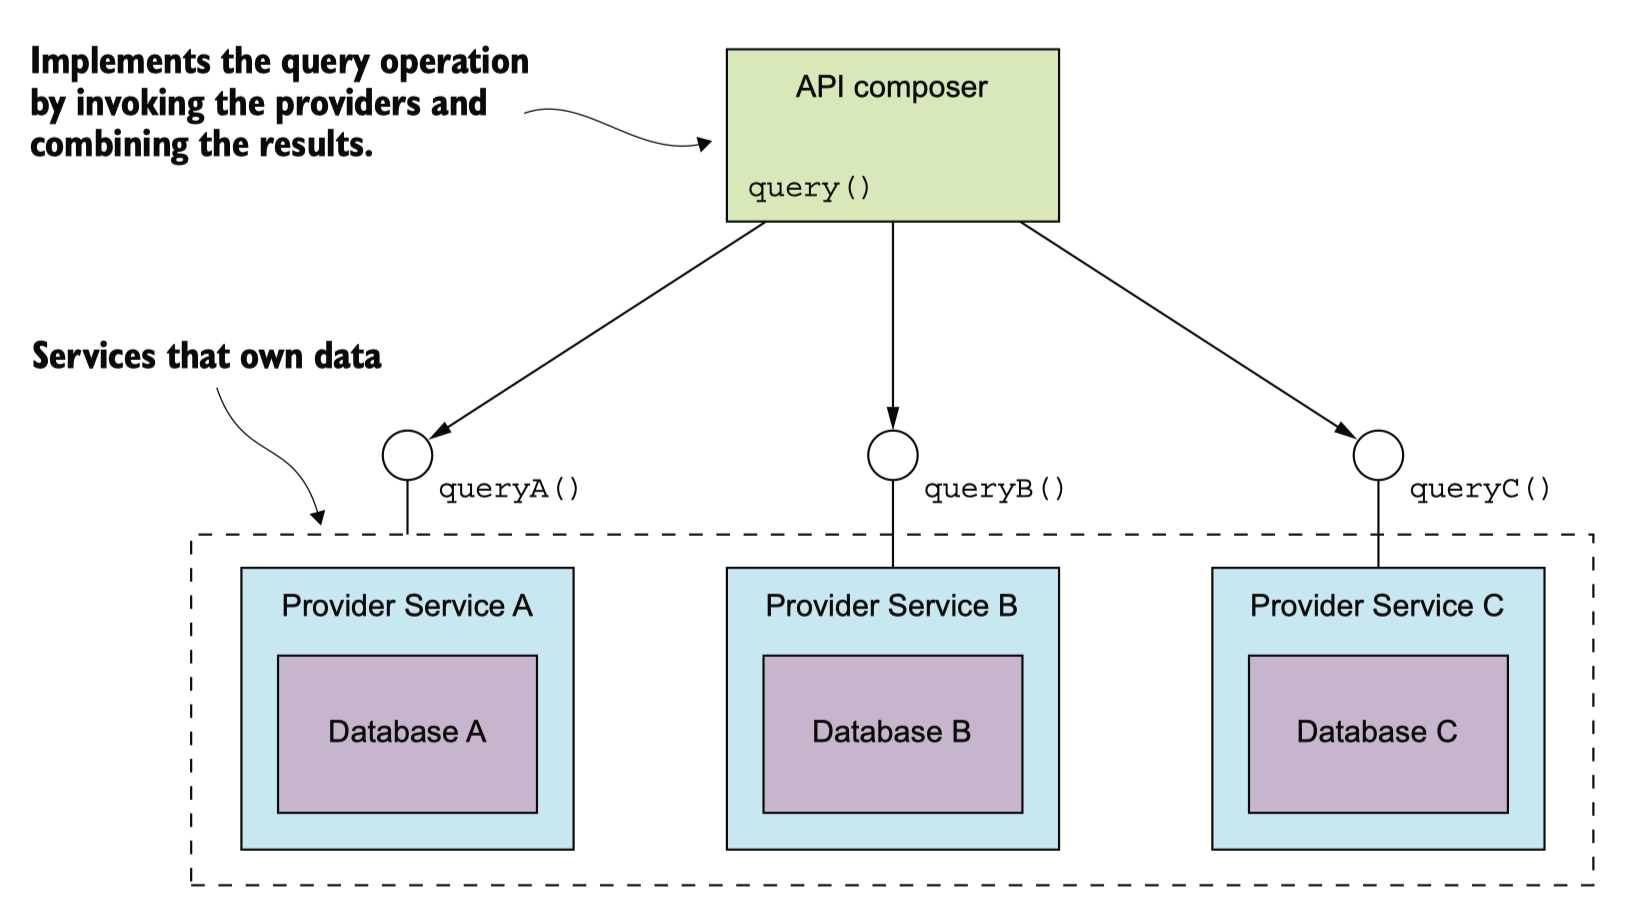
\includegraphics[width=3in]{jpeg/api-composition}
\caption{The API composition pattern implements an operation by querying the service providers and combining the results. \cite{microservices-patterns-api-composition}}
\label{cqrs}
\end{figure}

The role of API composer is usually taken by a service such as an API gateway, in which case the pattern is also called Gateway Aggregation \cite{gateway-aggregation}. This approach requires developing your own API gateway with a framework or library, instead of just configuring static files using an off-the-shelf API gateway such as Ambassador for Kubernetes\footnote{\url{https://www.getambassador.io/}}. 

This pattern can reduce the number of requests made to the services and improve application performance over high-latency networks, especially when caching techniques are applied.

However, the API composition pattern has several drawbacks. It can result in a very inefficient in-memory join of large datasets and it requires more computing and network resources, increasing the cost of running the application. Moreover, there is a risk that a query operation will return inconsistent data since it executes queries against multiple databases.

Lastly many queries can't be implemented using this pattern. Image an operation which retrieves a consumer’s order history. In contrast to replying with the details of a single order, it returns multiple orders from different services. Requesting orders from the services by ID is only practical if those services have a bulk fetch API, which is however unlikely. Requesting orders individually will, on the other hand, be inefficient because of excessive network traffic.

On the implementation side, an API composer should call provider services in parallel in order to minimize the response time for a query operation. Sometimes, though, an API composer needs the result of one service in order to invoke another one. The logic to efficiently execute a mixture of sequential and parallel service invocations can therefore be complex.

In order for an API composer to be maintainable as well as performant, it could use a reactive design based on Reactive streams (explained later) or some other equivalent abstraction, such as Futures or Promises depending on the programming language \cite{futures-and-promises}. Reactive streams and futures or promises make it possible to compose asynchronous operations or define a pipeline of operations to be invoked upon completion of the computation. This is in contrast to callback-heavy or more imperative direct blocking approaches.

Ultimately, whether you can use the API composition pattern to implement a particular query operation depends also on how the data is partitioned and the capabilities of the APIs exposed by the services that own the data. 

\subsection{CQRS pattern}

In contrast to the API composition pattern, the Command query responsibility segregation (CQRS) pattern \cite{cqrs-fowler} is more powerful as we shall explain, but it's also more complex. It maintains one or more view databases whose sole purpose is to support queries.

\begin{figure}[!htbp]
\centering
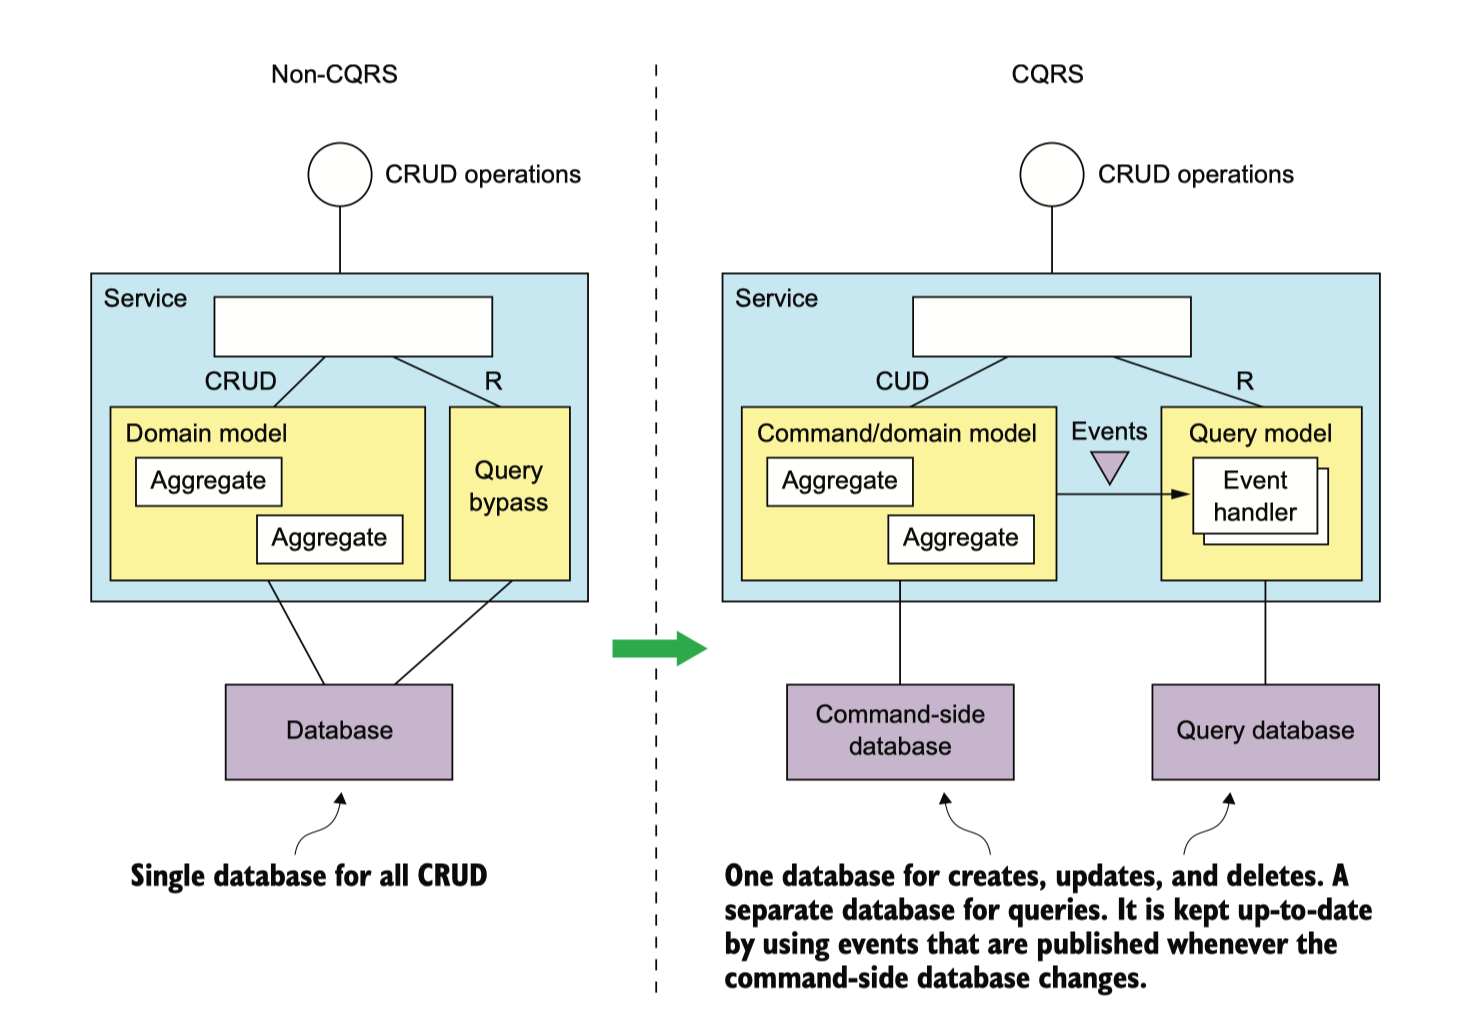
\includegraphics[width=3in]{jpeg/cqrs}
\caption{On the left is the not-CQRS version of the service, and on the right is the CQRS version. \cite{microservices-patterns-cqrs}}
\label{cqrs}
\end{figure}

Command Query Responsibility Segregation, as the name suggests, is all about segregation, or the separation of concerns. As figure \ref{cqrs} shows, in a non-CQRS service, the create, read, update and delete (CRUD) operations are typically implemented by a domain model that’s mapped to a database. An Object-Relational Mapping (ORM) \cite{orm} is a common technique in these cases, although for performance reasons, a few queries might bypass the domain model and access the database directly. On the other hand, a CQRS service splits a persistent data model and the modules that use it into two parts: the command side and the query side.

\begin{itemize}
  \item The write side (or command side) implements create, update, and delete operations (CUD) managing its own database and ensuring business rules. It may also handle simple queries, such as non-join, primary key-based queries. The command side publishes events whenever its data changes;
  \item The read side (or query side) is separate to the write side, which means different object models, probably running in different processes, perhaps on separate hardware. The query side handles only read operation. It subscribes to events produced by the write side and uses them to build and maintain a model that is suitable for answering client queries. Consequently, it uses whatever kind of database makes sense for the queries that it must support. The read side can be seen as an implementation of the Reporting Database pattern \cite{reporting-database}.
\end{itemize}

CQRS enables the efficient implementation of queries that retrieve data owned by multiple services, especially compared to the API composition pattern which sometimes results in expensive, inefficient in-memory joins.

Furthermore, separation of the read and write sides allows each to be scaled appropriately to match the workload. For example, query sides typically encounter a much higher demand than the write one.

CQRS also allows an application or service to efficiently implement a diverse set of queries. Attempting to support all queries using a single persistent data model is also often challenging and in some cases impossible. Even when a relational database has extensions to support a particular kind of query, using a specialized database is often more efficient. The CQRS pattern avoids the limitations of a single database by defining one or more read sides, each of which efficiently implements specific queries.

Another benefit is that CQRS defines separate code modules and database schemas for the command and query sides of a service. By separating concerns, the command side and query side are independent from each other and likely to be simpler and easier to maintain. The write side database can be refactored without needing to change to read databases.

Even though CQRS has several benefits, there are the significant additional operational complexity of managing and operating the extra data stores, which might even be of different types. Besides, as you might expect, there’s a delay between when the command side publishes an event and when the query side processes that event and updates its read model. A client application that updates a model using a write operation and then immediately queries a view may see the previous version of the data. It is likely though that the system has settled for eventual consistency, discussed in next section about distributed transactions.

On the implementation side, applying the CQRS pattern does not actually mandate that you use different data stores for write and read sides, or that you use any particular persistence technology such as a relational database, NoSQL store, or event store. Nevertheless, a NoSQL database is often a good choice for a CQRS read side, which can leverage its strengths like ease of scaling and ignore its weaknesses. A CQRS view is unaffected by the limitations of a NoSQL database, because it only uses simple transactions and executes a fixed set of queries without the need for relational joins. Actually you don't need to normalize the database, because it's read-only and the records can duplicate data as much as needed to make queries easier.

Although CQRS does not require messaging, it's common to use messaging to process commands and publish update events. Messages also allow CQRS write part to handle commands asynchronously from a queue, rather than being processed synchronously, making the service itself asynchronous.

In that case, the application must handle message failures or duplicate messages. A command or event handler should be idempotent whenever possible, that is duplicate events results in the same correct outcome. For instance, an events which cancels an order can be repeated multiple times with the same result. In other cases events can be structured differently to be idempotent.

\begin{lstlisting}
{
  "likingUser": 2,
  "restaurantId": 1
}
\end{lstlisting}

A service could be subscribed to this \texttt{ThumbsUpEvent} event and increment a thumbs-up counter for a restaurant, but if the same event will arrive twice the the counter will be incremented twice as well. To solve this problem, the event structure can be changed as follows:

\begin{lstlisting}
{
  "likingUser": 2,
  "restaurantId": 1,
  "totalLikes": 320
}
\end{lstlisting}

Thanks to that, no matter how many times event will arrive, the resulting state will be the same as only one copy arrived.

Unfortunately idempotent events make your system vulnerable for simultaneous events. Two \texttt{ThumbsUpEvent} could be published at the same time by two different users, however they will carry the same \texttt{totalLikes}. Out-of-order events are likewise troublesome: two events could be published sequentially but if they will arrive in the wrong order then the system will remain inconsistent.

As demonstrated, an idempotent event is not feasible most of the time. A non-idempotent event handler must instead detect and discard duplicate events by recording the ids of events that it has already processed. One viable solution is to keep the history of IDs of all events that they have already seen. Theoretically, a CQRS read side should keep a full history of events, but in practice, the last couple of hours should be sufficient.

CQRS provide a lot of benefits when it comes to the scalability of data queries. Unfortunately, it doesn’t come for free and the attached costs may be severely underestimated causing significant decrease in productivity .

However, since we have seen how to query data spanning multiple services, we proceed to analyse more complex transactions that involve several services.

\section{Distributed transactions}

ACID (Atomicity, Consistency, Isolation, Durability) transactions greatly simplify the job of the developer by providing the illusion that each transaction has exclusive access to the data. In a microservice architecture, a single service can still use ACID transactions for local operations. The challenge, however, lies in implementing transactions for operations that update data owned by multiple services, each of which has its own database, without violating consistency.

By consistency, we mean state consistency that is a transaction preserves all the database rules, such as  referential integrity or, for example, when transferring money from one account to another the total amount held in both accounts should not change. This is not to be confused with the copy consistency in the CAP theorem \cite{acid-cap}, which refers to having all the copies of the data up-to-date, a subset of the former consistency.

The traditional approach to maintaining data consistency across multiple services or databases is to use distributed transactions. The de facto standard for distributed transaction management is the X/Open Distributed Transaction Processing (DTP) Model \cite{dtp}, which uses two-phase commit (2PC) to ensure that all participants in a transaction either commit or rollback. 

Several problems arise however when a 2PC protocol is used in a system where network and hardware failures occur or a server could just crash. For instance, the coordinator, as well as the participants, have states in which they block waiting for incoming messages \cite{distributed-systems-2pc}. For that reason, the main problem with traditional distributed transactions is that they reduce availability. For a distributed transaction to commit, all the participating services must be available.

The overall availability is the product of the availability of all of the participants in the transaction. If a distributed transaction involves four services that are 99.5\% available, then the overall availability is 98\%, which is significantly less. Each additional service involved in a distributed transaction further reduces availability.

On top of that, the famous CAP theorem provides another proof of the unsuitability of distributed transactions:

\begin{quote}
It is impossible for a distributed data store to simultaneously provide more than two out of the following three guarantees: consistency, availability, partition tolerance.

\hfill Eric Brewer
\end{quote}

The original theorem refers to copy consistency, but ACID consistency also cannot be maintained across partitions. 

Although the formulation was misleading and has been revisited \cite{acid-cap}, it remains true that the CAP theorem prohibits perfect availability and consistency in the presence of network partitions. But the three properties are continuous values other than binary. Availability is already expressed as a range from 0 to 100\%, but there are also many levels of consistency and even partitions usually affect portions of a system, not a globally.

The modern CAP goal tries to maximize combinations of consistency and availability that make sense for the specific application. Such an approach incorporates plans for operation during a partition to mantain availability and for recovery afterward, for keep consistency.

As a matter of fact, many systems nowadays drop perfect consistency in favour of eventual consistency \cite{consistency-vs-availability}, availability and partition tolerance. Temporary inconsistency can be tolerated for two reasons: for improving read and write performance under highly concurrent conditions and for handling partition cases where a majority model would render part of the system unavailable even though the nodes are up and running. Clearly, partition recovery will need to restore ACID consistency since maintaining invariants during partitions might be impossible.

It is clear at this point that to solve the complex problem of maintaining data consistency in a microservice architecture, an application must use a different mechanism that builds on top of the asynchronous CQRS services. CQRS services are already partition tolerant since commands and queries are handled without the need of external services and events are usually implemented as asynchronous messages. What is missing though is a mechanism to keep the consistency and plan for recovery if a partition occurs. This is where the saga pattern comes in.

\section{The saga pattern}

A saga is a sequence of local transactions. Each local transaction updates data within a single service using the familiar ACID transaction.

A saga is initiated by a command event and it reacts to subsequent command events, generating new ones and thus allowing command handlers to be kept independent.

While handling a request, the service doesn’t synchronously interact with any other service. Instead, it asynchronously sends messages to other services which are not required to be available at the same time. Eventually, any unavailable service will come back up and process queued messages.

\begin{figure}[!htbp]
\centering
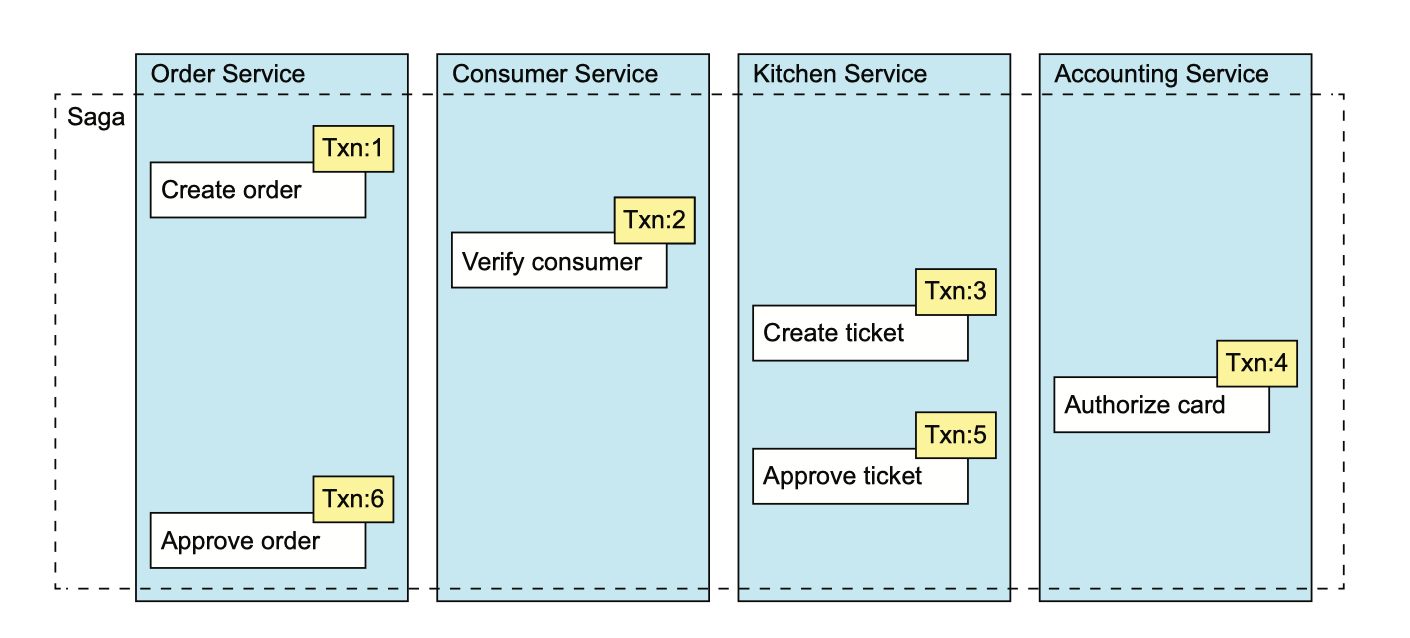
\includegraphics[width=3in]{jpeg/order-saga}
\caption{Creating an Order using a saga. \cite{microservices-patterns-saga}}
\label{order_saga}
\end{figure}

The example saga used throughout this section is the \texttt{Create Order Saga}, which is shown in Figure \ref{order_saga}. The saga’s first local transaction is initiated by a command event to create an order. The other five local transactions are each triggered by command events signalling the completion of the previous one.

This saga consists of the following local transactions:

\begin{enumerate}
  \item Order Service: it creates an order in an \texttt{APPROVAL\_PENDING} state;
  \item Consumer Service: it verifies that the consumer can place an order;
  \item Kitchen Service: it validates order details and create a ticket in the \texttt{CREATE\_PENDING} state;
  \item Accounting Service: it authorises the consumer’s credit card;
  \item Kitchen Service: it changes the state of the ticket to \texttt{AWAITING\_ACCEPTANCE};
  \item Order Service: it changes the state of the order to \texttt{APPROVED}.
\end{enumerate}

\subsection{Compensating transactions}

A great feature of traditional ACID transactions is that the business logic can easily roll back a transaction if it detects the violation of a business rule. Unfortunately, sagas can’t be automatically rolled back, because each step commits its changes to the local database. 

To see how compensating transactions are used, imagine a scenario where the authorisation of the consumer’s credit card fails. In this scenario, the saga executes the following local transactions:

\begin{enumerate}
  \item Order Service: it creates an order in an \texttt{APPROVAL\_PENDING} state;
  \item Consumer Service: it verifies that the consumer can place an order;
  \item Kitchen Service: it validates order details and creates a ticket in the \texttt{CREATE\_PENDING} state;
  \item Accounting Service: it authorises consumer’s credit card, which fails;
  \item Kitchen Service: it changes the state of the ticket to \texttt{CREATE\_REJECTED};
  \item Order Service: it changes the state of the order to \texttt{REJECTED}.
\end{enumerate}

The fifth and sixth steps are compensating transactions that undo the updates made by the Kitchen Service and Order Service, respectively.

A saga’s coordination logic is therefore responsible for sequencing the execution of both forward and compensating transactions. \cite{microservices-patterns-saga}

\subsection{Lack of isolation}

The I in ACID stands for isolation. The isolation property of ACID transactions ensures that the outcome of executing multiple transactions concurrently is the same as if they were executed in some serial order. The database provides the illusion that each ACID transaction has exclusive access to the data.

The challenge of using sagas is that they lack the isolation property of ACID transactions. That’s because the updates made by each of a saga’s local transactions are immediately visible to other sagas once that transaction commits. This behaviour can cause two problems. First, other sagas can change the data accessed by the saga while it’s executing. And second, other sagas can read its data before the saga has completed its updates and consequently can be exposed to inconsistent data.

This lack of isolation potentially causes database \textit{anomalies}. An anomaly is when a transaction reads or writes data in a way that it wouldn’t if transactions were executed one at time. When an anomaly occurs, the outcome of executing sagas concurrently is different than if they were executed serially.

The lack of isolation can cause the following three anomalies \cite{microservices-patterns-anomalies}:

\begin{enumerate}
  \item \textit{Lost updates}: one saga overwrites without reading changes made by another saga;
  \item \textit{Dirty reads}: a transaction or a saga reads the updates made by a saga that has not yet completed;
  \item \textit{Fuzzy/non-repeatable reads}: two different steps of one saga read the same data and get different results because another saga has made updates;
\end{enumerate}

It’s then the responsibility of the developer to adopt a set of countermeasures for handling anomalies caused by lack of isolation that either prevent one or more anomalies or minimize their impact on the business. \cite{semantic-acid}

One example of countermeasure is the usage of semantic locks: a saga’s compensatable transaction sets a flag in any record that it creates or updates. The flag indicates that the record isn’t committed and could potentially change. The flag can either be a lock that prevents other transactions from accessing the record or a warning that indicates that other transactions should treat that record with suspicion.

\subsection{Reliable events}

It’s essential for the database update and the publishing of the event to happen atomically. Consequently, to communicate reliably, the saga participants must use transactional messaging. Otherwise, a service might update the database and then crash, for example, before sending the message. If the service doesn’t perform these two operations atomically, a failure could leave the system in an inconsistent state.

A straightforward way to reliably publish messages is to apply the Transactional outbox pattern. This pattern uses a database table as a temporary message queue, where the service inserts messages. Atomicity is guaranteed because this is a local ACID transaction. Then, an effortless way to publish the messages is to poll the table for unpublished messages although frequently polling the database can be expensive.

A sophisticated solution is to tail the database transaction log (also called the commit log). Every committed update made by an application is represented as an entry in the database’s transaction log. A transaction subscriber can read the transaction log and publish each change as a message to the message broker. \cite{log-tailing}

\section{Communication}

As we have seen with the previous patterns, the services within a microservice architecture must frequently collaborate in order to complete a saga or to handle a query request. Because service instances are typically processes running on multiple machines, they must interact using Inter-Process Communication (IPC).

The choice of IPC mechanism is an important architectural decision since it can impact application availability and it intersects with transaction management. As we have seen with the saga pattern, we favour loosely coupled services that communicate with one another using asynchronous messaging.

Synchronous protocols such as REST and RPC are used mostly to communicate with other applications. The problem with REST is that it’s a synchronous protocol: an HTTP client must wait for the service to send a response. Whenever services communicate using a synchronous protocol, the availability of the application is reduced.

\subsection{Message Queuing}

On the other hand, the basic idea behind a message-queuing system is that applications communicate by inserting messages in specific queues by using a message broker, an infrastructure service through which all messages flow.

A critical aspect of message-queuing systems is that a sender is generally given only the guarantees that its message will eventually be inserted in the recipient’s queue. No guarantees are given about when, or even if the message will actually be read, which is completely determined by the behaviour of the recipient. These semantics permit communication to be \textit{loosely coupled in time}.

When selecting a message broker, you have various factors to consider, including the following:

\begin{itemize}
  \item Messaging ordering: does the message broker preserve ordering of messages?
  \item Delivery guarantees: what kind of delivery guarantees does the broker make?
  \item Persistence: are messages persisted to disk and able to survive broker crashes?
  \item Durability: if a consumer reconnects to the message broker, will it receive the messages that were sent while it was disconnected?
  \item Scalability: how scalable is the message broker?
  \item Latency: what is the end-to-end latency?
\end{itemize}

Each broker makes different trade-offs. For example, a very low-latency broker might not preserve ordering, make no guarantees to deliver messages and only store messages in memory. A messaging broker that guarantees delivery and reliably stores messages on disk will probably have higher latency. Which kind of message broker is the best fit depends on your application’s requirements. \cite{microservices-patterns-broker}

After picking the proper broker solution for your application, we can see how the saga orchestrator communicates with the participants using async reply-style interaction based on message queues. To execute a saga step, it sends a command message to a participant telling what operation to perform. After the saga participant has performed the operation, it sends a reply message to the orchestrator. The orchestrator then processes the message and determines which saga step to perform next.

\begin{figure}[!htbp]
\centering
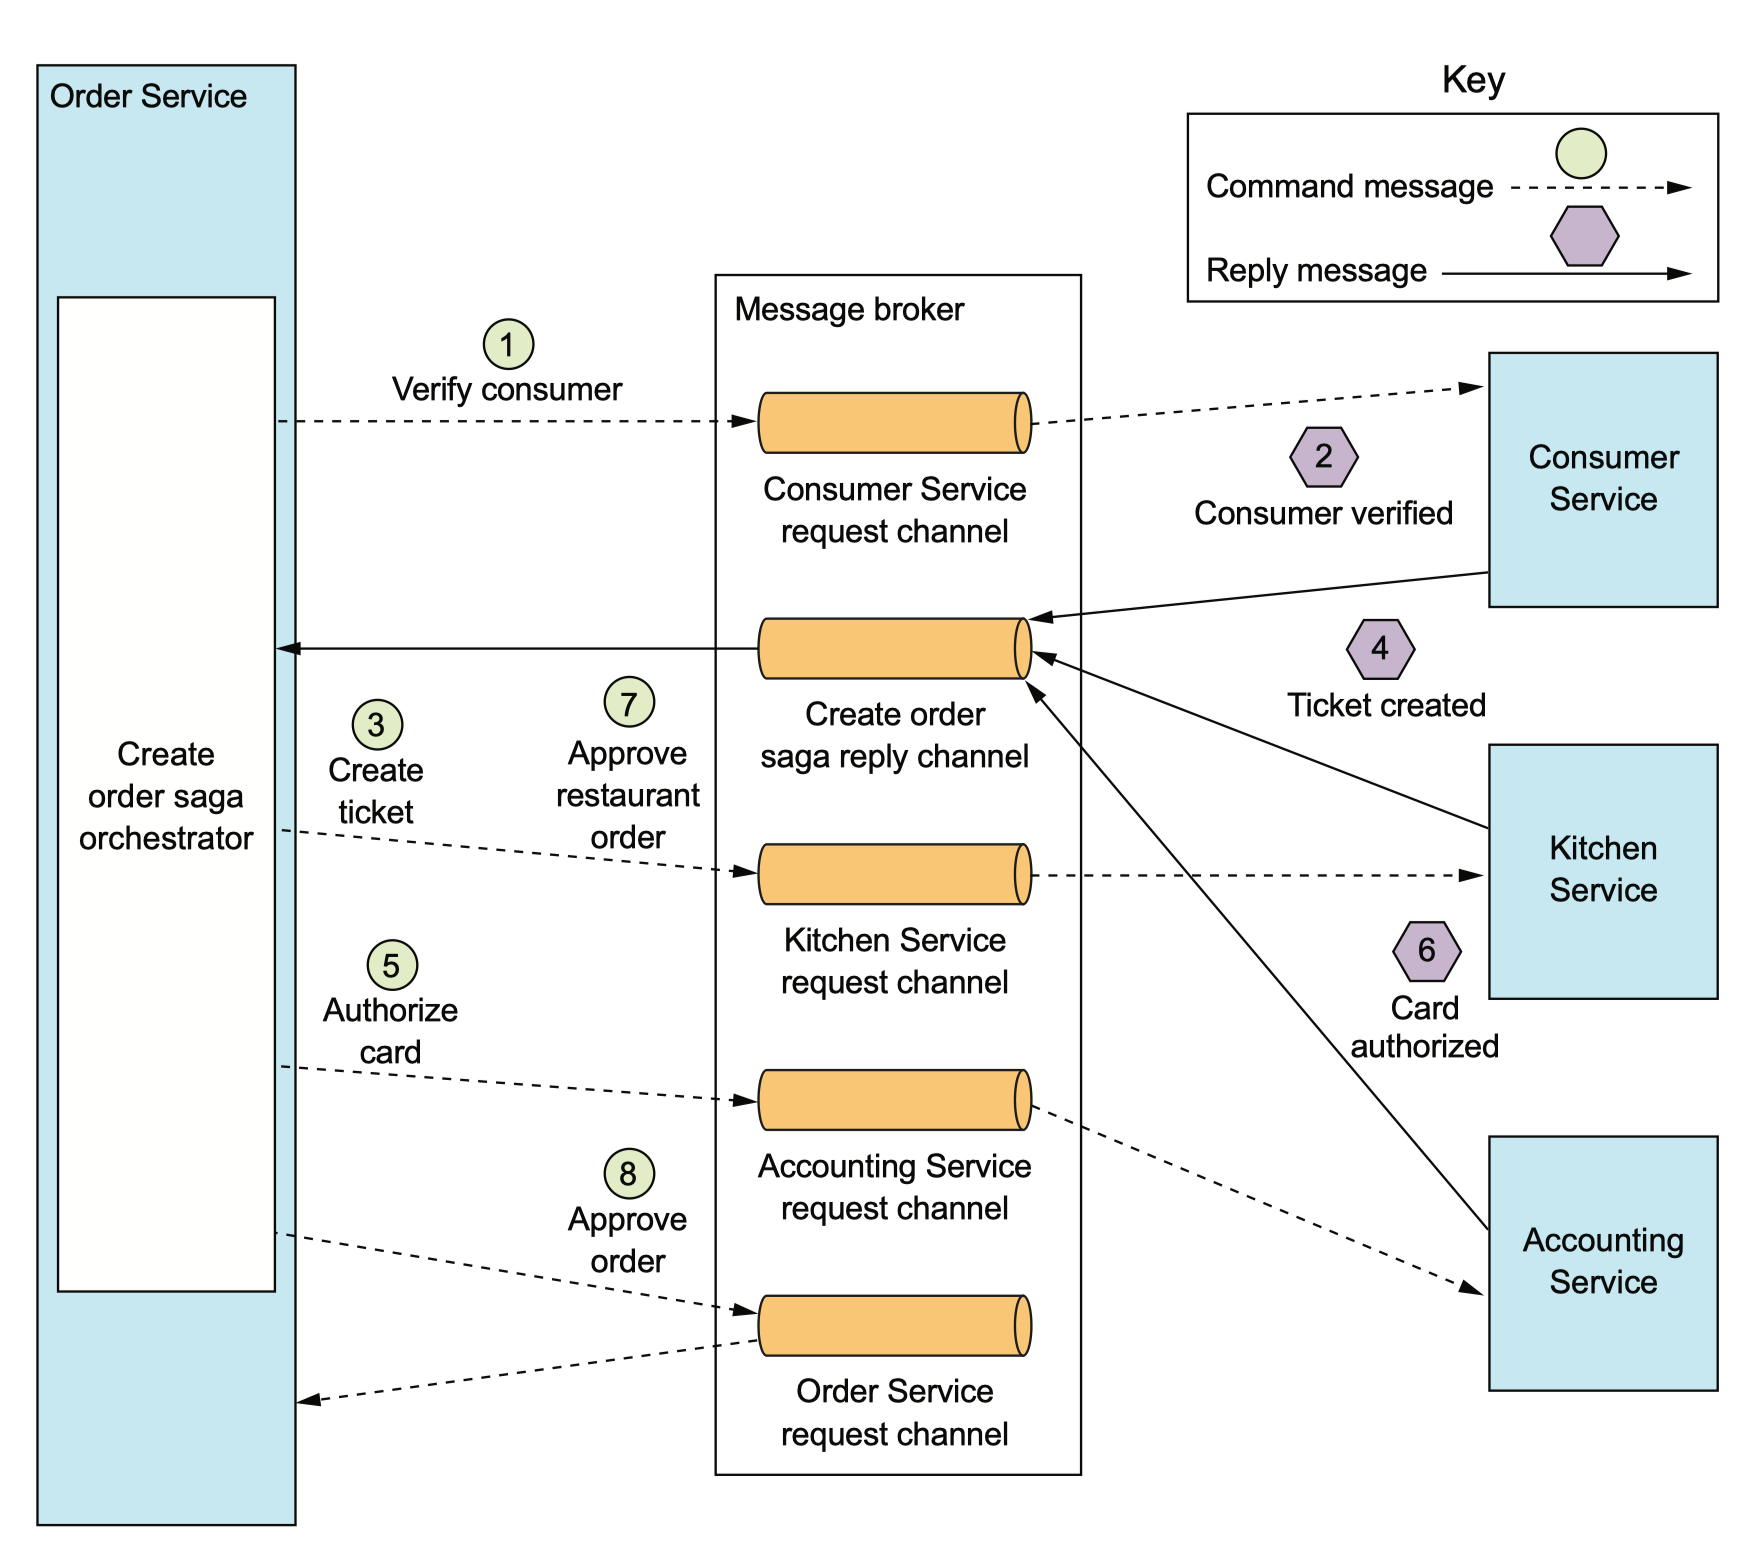
\includegraphics[width=3in]{jpeg/orchestrator-saga}
\caption{Order Service implements a saga orchestrator, which invokes the saga participants using asynchronous request/response. \cite{microservices-patterns-saga}}
\label{orchestrator_saga}
\end{figure}

Although CQRS does not require messaging, it's common to use messaging to process commands and publish update events.
Clients typically send commands to the domain through a messaging system such as a queue.
Messages also allow CQRS write part to handle commands asynchronously from a queue, rather than being processed synchronously.

\section{Technologies}

https://github.com/chimurai/http-proxy-middleware but doesn't have rate limiting and other edge functions

\subsection{Reactive Programming}

Example of using forkJoin for OrderDetails API composition.

\subsection{Promises and Futures}

Error handling compared to callbacks.

Performance problems of Reactive streams and Promises.

\subsection{Event bus}

% An example of a floating figure using the graphicx package.
% Note that \label must occur AFTER (or within) \caption.
% For figures, \caption should occur after the \includegraphics.
% Note that IEEEtran v1.7 and later has special internal code that
% is designed to preserve the operation of \label within \caption
% even when the captionsoff option is in effect. However, because
% of issues like this, it may be the safest practice to put all your
% \label just after \caption rather than within \caption{}.
%
% Reminder: the "draftcls" or "draftclsnofoot", not "draft", class
% option should be used if it is desired that the figures are to be
% displayed while in draft mode.
%
%\begin{figure}[!t]
%\centering
%\includegraphics[width=2.5in]{myfigure}
% where an .eps filename suffix will be assumed under latex, 
% and a .pdf suffix will be assumed for pdflatex; or what has been declared
% via \DeclareGraphicsExtensions.
%\caption{Simulation Results.}
%\label{fig_sim}
%\end{figure}

% Note that IEEE typically puts floats only at the top, even when this
% results in a large percentage of a column being occupied by floats.


% An example of a double column floating figure using two subfigures.
% (The subfig.sty package must be loaded for this to work.)
% The subfigure \label commands are set within each subfloat command,
% and the \label for the overall figure must come after \caption.
% \hfil is used as a separator to get equal spacing.
% Watch out that the combined width of all the subfigures on a 
% line do not exceed the text width or a line break will occur.
%
%\begin{figure*}[!t]
%\centering
%\subfloat[Case I]{\includegraphics[width=2.5in]{box}%
%\label{fig_first_case}}
%\hfil
%\subfloat[Case II]{\includegraphics[width=2.5in]{box}%
%\label{fig_second_case}}
%\caption{Simulation results.}
%\label{fig_sim}
%\end{figure*}
%
% Note that often IEEE papers with subfigures do not employ subfigure
% captions (using the optional argument to \subfloat[]), but instead will
% reference/describe all of them (a), (b), etc., within the main caption.


% An example of a floating table. Note that, for IEEE style tables, the 
% \caption command should come BEFORE the table. Table text will default to
% \footnotesize as IEEE normally uses this smaller font for tables.
% The \label must come after \caption as always.
%
%\begin{table}[!t]
%% increase table row spacing, adjust to taste
%\renewcommand{\arraystretch}{1.3}
% if using array.sty, it might be a good idea to tweak the value of
% \extrarowheight as needed to properly center the text within the cells
%\caption{An Example of a Table}
%\label{table_example}
%\centering
%% Some packages, such as MDW tools, offer better commands for making tables
%% than the plain LaTeX2e tabular which is used here.
%\begin{tabular}{|c||c|}
%\hline
%One & Two\\
%\hline
%Three & Four\\
%\hline
%\end{tabular}
%\end{table}


% Note that IEEE does not put floats in the very first column - or typically
% anywhere on the first page for that matter. Also, in-text middle ("here")
% positioning is not used. Most IEEE journals/conferences use top floats
% exclusively. Note that, LaTeX2e, unlike IEEE journals/conferences, places
% footnotes above bottom floats. This can be corrected via the \fnbelowfloat
% command of the stfloats package.



\section{Conclusion}

We started the paper by showing the reasons behind a database-per-service solution in a microservice architecture. Unfortunately, no technology is a silver bullet and this solution has several significant drawbacks and it adds risky complexity.

One issue is that developers must deal with the additional complexity of managing databases in a distributed system. It's crucial to use an interprocess communication pattern aware of the asynchronous nature of the communication and the transience of the system, such as message queuing. Missing a message like a command event could indeed leave the system in an inconsistent state.

Moreover, implementing use cases that span multiple services requires the use of unfamiliar techniques like CQRS and sagas. One big obstacle that developers will have to face when adopting microservices is moving from a single database with ACID transactions to a multi-database architecture with ACD sagas, because they’re used to the simplicity of the ACID transaction model.

All the patterns explored in this paper require a significant mental leap, so they shouldn't be tackled unless the benefit is worth the jump. Having a database-per-service might be needed on specific portions of a system and not the system as a whole, based on the different scaling/usage characteristics. In this way, some portions can use a shared database without encountering all the complexities seen before, while others will benefit  from a separated data store and the previous patterns. The former services may no be truly independent microservices, more just services in Service-Oriented-Architecture \cite{soa}, but it is crucial for development teams to understand how to balance the cost and benefits of microservices. 

% conference papers do not normally have an appendix





% trigger a \newpage just before the given reference
% number - used to balance the columns on the last page
% adjust value as needed - may need to be readjusted if
% the document is modified later
%\IEEEtriggeratref{8}
% The "triggered" command can be changed if desired:
%\IEEEtriggercmd{\enlargethispage{-5in}}

% references section

% can use a bibliography generated by BibTeX as a .bbl file
% BibTeX documentation can be easily obtained at:
% http://www.ctan.org/tex-archive/biblio/bibtex/contrib/doc/
% The IEEEtran BibTeX style support page is at:
% http://www.michaelshell.org/tex/ieeetran/bibtex/
%\bibliographystyle{IEEEtran}
% argument is your BibTeX string definitions and bibliography database(s)
%\bibliography{IEEEabrv,../bib/paper}
%
% <OR> manually copy in the resultant .bbl file
% set second argument of \begin to the number of references
% (used to reserve space for the reference number labels box)
\begin{thebibliography}{1}

\bibitem{exploring-microservices}
Alberto Simioni, Tullio Vardanega, "In Pursuit of Architectural Agility: Experimenting with Microservices" in \textit{2018 IEEE International Conference on Services Computing (SCC)}, July 2018. [Online] Available: https://ieeexplore.ieee.org/document/8456408
\bibitem{ebay-architecture}
Randy Shoup, "The eBay Architecture: Striking a Balance between Site Stability, Feature Velocity, Performance, and Cost", pp. 21-22. [Online]. Available: https://www.slideshare.net/RandyShoup/the-ebay-architecture-striking-a-balance-between-site-stability-feature-velocity-performance-and-cost
\bibitem{database-per-service}
Chris Richardson, "Database per service" in "Microservice Architecture". [Online]. Available: https://microservices.io/patterns/data/database-per-service.html
\bibitem{microservices-patterns-api-composition}
Chris Richardson, "Querying using the API composition pattern" in "Microservices Patterns", pp. 221-228, October 2018.
\bibitem{gateway-aggregation}
Microsoft Developer Network, "Gateway Aggregation pattern" in "Cloud Design Patterns". [Online]. Available: https://docs.microsoft.com/en-us/azure/architecture/patterns/gateway-aggregation
\bibitem{futures-and-promises}
Kisalaya Prasad, Avanti Patil, Heather Miller, "Futures and Promises" in "Programming Models for Distributed Computing". [Online]. Available: http://dist-prog-book.com/chapter/2/futures.html
\bibitem{cqrs-fowler}
Martin Fowler, "CQRS". [Online]. Available: http://hibernate.org/orm/what-is-an-orm/
\bibitem{orm}
Hibernate, "What is Object/Relational Mapping". [Online]. Available: https://martinfowler.com/bliki/CQRS.html
\bibitem{microservices-patterns-cqrs}
Chris Richardson, "Overview of CQRS" in "Microservices Patterns", pp. 232-233, October 2018.
\bibitem{reporting-database}
Martin Fowler, "ReportingDatabase". [Online]. Available: https://martinfowler.com/bliki/ReportingDatabase.html
\bibitem{microservices-patterns-saga}
Chris Richardson, "Using the Saga pattern to maintain data consistency" in "Microservices Patterns", pp. 114-117, October 2018.
\bibitem{microservices-patterns-anomalies}
Chris Richardson, "Handling the lack of isolation" in "Microservices Patterns", pp. 126-131, October 2018.
\bibitem{microservices-patterns-broker}
Chris Richardson, "Overview of broker-based messaging" in "Microservices Patterns", pp. 92, October 2018.
\bibitem{distributed-systems-2pc}
Maarten van Steen, Andrew S. Tanenbaum, "Distributed Systems", pp. 483-490, February 2017.
\bibitem{acid-cap}
Eric Brewer, "CAP Twelve Years Later: How the "Rules" Have Changed". [Online]. Available: https://www.infoq.com/articles/cap-twelve-years-later-how-the-rules-have-changed/
\bibitem{dtp}
Microsoft Developer Network, "X-Open Distributed Transaction Processing Standard". [Online]. Available: https://docs.microsoft.com/en-us/previous-versions/windows/desktop/ms686548(v\%3Dvs.85)
\bibitem{consistency-vs-availability}
Werner Vogels, "Eventually Consistent". [Online]. Available: https://queue.acm.org/detail.cfm?id=1466448
\bibitem{semantic-acid}
Lars Frank, Torben U. Zahle, "
Semantic ACID properties in multidatabases using remote procedure calls and update propagations". [Online]. Available: https://dl.acm.org/citation.cfm?id=284472.284478
\bibitem{log-tailing}
Oded Shopen, "Listen to Yourself: A Design Pattern for Event-Driven Microservices". [Online]. Available: https://medium.com/@odedia/listen-to-yourself-design-pattern-for-event-driven-microservices-16f97e3ed066
\bibitem{soa}
Microsoft Developer Network, "Service Oriented Architecture (SOA)" in "SOA in the Real World". [Online]. Available: https://web.archive.org/web/20160206132542/https://msdn.microsoft.com/en-us/library/bb833022.aspx

\end{thebibliography}




% that's all folks
\end{document}


